\textbf{COLUNI 2022 -- Questão 37}\par\medskip As imagens a seguir colocam em foco questões relativas à população indígena brasileira, em diferentes momentos de nossa história, problematizando acontecimentos em torno de temas como proteção aos indígenas, direitos de acesso e permanência à terra, extermínio de populações, conflitos com grupos locais e regionais, diversidade cultural, mobilização e resistência, entre outros. Esses debates e discussões perpassaram a história brasileira do século XX e as primeiras décadas do século XXI.

\par

\begin{minipage}[t]{0.48\linewidth}\centering
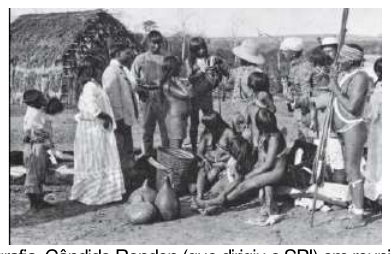
\includegraphics[width=\linewidth]{static/simulados/coluni/figuras/2022/questao-37/figura-1.png}\par
Na fotografia, Cândido Rondon (que dirigiu o SPI) em reunião com indígenas do povo Parisí no Mato Grosso. Imagem do início do século XX, sem data definida. Museu do índio, Rio de Janeiro. \textit{In:} CONTRIM, Gilberto; RODRIGUES, Jaime. \textit{Historiar}, 9º ano: ensino fundamental, anos finais. 3. ed. São Paulo: Editora Saraiva, 2018, p. 28.
\end{minipage}\hfill
\begin{minipage}[t]{0.48\linewidth}\centering
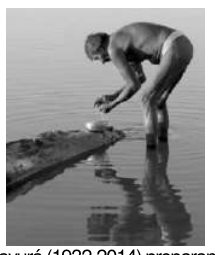
\includegraphics[width=\linewidth]{static/simulados/coluni/figuras/2022/questao-37/figura-2.png}\par
Pajé Takumã Kamayurá (1932-2014) preparando uma infusão de plantas. Tukumã lutou pela criação do Parque Indígena do Xingu, em 1961, e pela união de diferentes povos em torno dessa causa. Parque indígena do Xingu, município de Querência, Mato Grosso. Fotografia de 2011. \textit{In:} CONTRIM, Gilberto; RODRIGUES, Jaime. \textit{Historiar}, 9º ano: ensino fundamental, anos finais. 3. ed. São Paulo: Editora Saraiva, 2018, p. 145. (Adaptado)
\end{minipage}

\medskip

\begin{minipage}[t]{0.48\linewidth}\centering
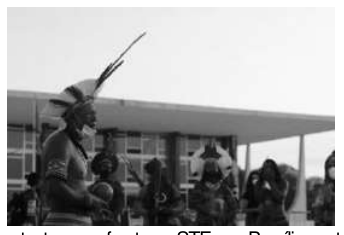
\includegraphics[width=\linewidth]{static/simulados/coluni/figuras/2022/questao-37/figura-3.png}\par
Indígenas protestam em frente ao STF, em Brasília contra o marco temporal para demarcação de terras, nesta quarta-feira (25). — Foto: Carolina Cru/G1. 25/08/2021. Disponível em: https://g1.globo.com/google/amp/df/distrito-federal/noticia/2021/08/25/indigenas-voltam-a-protestar-em-brasilia-contra-marco-temporal-para-demarcacao-de-terras.ghtml. Acesso em: 17 set. 2021.
\end{minipage}\hfill
\begin{minipage}[t]{0.48\linewidth}\centering
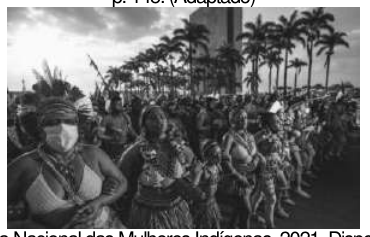
\includegraphics[width=\linewidth]{static/simulados/coluni/figuras/2022/questao-37/figura-4.png}\par
2.ª Marcha Nacional das Mulheres Indígenas, 2021. Disponível em: https://redecerrado.org.br/mulheres-indigenas-ocupam-brasilia-para-reflorestar-mentes/. Acesso em: 11 ago. 2021.
\end{minipage}

\par

Com relação aos debates e às discussões no Brasil sobre povos indígenas, ao longo do século XX e primeiras décadas do século XXI, e a garantia de seus direitos, analise as afirmativas abaixo:

\par

I. O Serviço de Proteção aos Índios (SPI), criado em 1910 e dirigido por Cândido Mariano da Silva Rondon, com a finalidade de proteger os nativos, preservar suas terras e culturas, constituiu-se a primeira política governamental de grande sucesso direcionada aos povos indígenas.\par
II. O Parque Indígena do Xingu é considerado uma das mais bem-sucedidas reservas indígenas do mundo, mas vem sendo afetado pelo crescimento das regiões circunvizinhas, pelo acelerado processo de deterioração ambiental e pelos conflitos em torno da biodiversidade de seu território.\par
III. A Constituição Federal de 1988 definiu que as terras indígenas são bens da União, garantiu o usufruto dessas terras aos nativos, e devia ainda demarcar as terras até 1993, o que não ocorreu em sua totalidade, gerando, até hoje, conflitos em torno do processo de demarcação.\par
IV. A expansão do movimento indígena a partir dos anos 1970, com o crescimento do número e da diversidade de organizações conduzidas pelos próprios nativos, é sinal de um protagonismo indígena que contribuiu para a formulação de políticas voltadas para esses povos.

\par

Está CORRETO o que se afirma apenas em:

\par

a) I, III e IV.\par
b) I e II.\par
c) II.\par
d) II, III e IV.




